\documentclass[11pt,a4paper]{article}
\usepackage[T1]{fontenc}
\usepackage[utf8]{inputenc}
\usepackage{lmodern}
\usepackage[a4paper,margin=2.4cm]{geometry}
\usepackage{microtype}
\usepackage{setspace}
\usepackage{amsmath}
\usepackage{graphicx}
\usepackage{booktabs,tabularx}
\usepackage[table]{xcolor}
\usepackage{caption}
\usepackage{subcaption}
\usepackage{float}
\usepackage{enumitem}
\usepackage{titlesec}
\usepackage{fancyhdr}
\usepackage{lastpage}
\usepackage[hidelinks]{hyperref}

\graphicspath{{figs/}}
\setstretch{1.15}
\setlength{\parindent}{0pt}
\setlength{\parskip}{0.55em}
\captionsetup{font=small,labelfont=bf,labelsep=period}
\setlist{itemsep=0.15em,topsep=0.3em}
\titleformat{\section}{\normalfont\large\bfseries}{\thesection}{0.8em}{}
\titleformat{\subsection}{\normalfont\normalsize\bfseries}{\thesubsection}{0.8em}{}
\titlespacing*{\section}{0pt}{1.3em}{0.5em}
\titlespacing*{\subsection}{0pt}{0.9em}{0.3em}

\pagestyle{fancy}
\fancyhf{}
\fancyhead[L]{\small\itshape Dahal --- Fine-tuning vs.\ LLMs for Nepali sentiment}
\fancyhead[R]{\small\itshape Preprint, not peer reviewed}
\fancyfoot[C]{\small \thepage\ of \pageref{LastPage}}
\renewcommand{\headrulewidth}{0.4pt}

\begin{document}

\begin{center}
{\LARGE\bfseries Is fine-tuning still worth it for a low-resource language? A controlled comparison of XLM-RoBERTa, a small open LLM and a character n-gram baseline for Nepali tweet sentiment\par}
\vspace{1.0em}
{\large Subarna Dahal\par}
\vspace{0.3em}
{\small Lalitpur, Nepal\quad$\cdot$\quad \href{mailto:dahalsubarna9@gmail.com}{dahalsubarna9@gmail.com}\par}
{\small Code and results: \url{https://github.com/subarna007/nepali-sentiment-finetune-vs-llm}\par}
\vspace{0.3em}
{\small Version of 18 November 2026\par}
\end{center}
\vspace{0.4em}
\noindent\rule{\textwidth}{0.4pt}

{\small
\textbf{Abstract}

\textbf{Background.} Instruction-tuned large language models (LLMs) can classify text without any training, which raises a practical question for languages with few resources: is it still worth collecting labels and fine-tuning a model? Nepali, spoken by tens of millions of people but with little labelled data, is a useful test case.

\textbf{Methods.} I used NepCOV19Tweets, a public set of Nepali COVID-19 tweets labelled positive, neutral or negative. Exact duplicate tweets were removed before a stratified 80/10/10 split (26,764 training, 3,345 validation and 3,346 test tweets), so no tweet appears in both training and test data. On the same test set I compared a character 1--4-gram TF-IDF model with logistic regression, XLM-RoBERTa-base fine-tuned on the full training set, and Qwen2.5-3B-Instruct used zero-shot and with two examples per class in the prompt. Macro-F1 was the main metric, with 95\% bootstrap intervals and McNemar tests on paired predictions.

\textbf{Results.} Fine-tuned XLM-RoBERTa reached a macro-F1 of 0.707 (95\% CI 0.688--0.725), ahead of the TF-IDF baseline at 0.657 (0.640--0.675; paired difference 0.051, 0.030--0.072; McNemar $p<10^{-18}$). The LLM reached 0.480 (0.462--0.498) zero-shot and 0.539 (0.520--0.557) with six examples, below the baseline in both settings. The LLM's errors were biased rather than random: zero-shot it labelled 581 of 1,360 negative tweets as positive, and with examples the bias flipped towards negative. Neutral was the hardest class for every method (F1 at most 0.49), and all methods did worse on longer tweets.

\textbf{Conclusions.} For Nepali sentiment, a fine-tuned 278M-parameter encoder clearly beats a 3B-parameter LLM used without training, and even a character n-gram model does. With a few thousand labels available, fine-tuning remains the better choice. The weak neutral class points to label ambiguity that no model choice fixes.

\textbf{Keywords:} Nepali; sentiment analysis; low-resource languages; XLM-RoBERTa; large language models; zero-shot; few-shot; evaluation\par
}
\noindent\rule{\textwidth}{0.4pt}

\section{Introduction}

Most NLP progress is measured on English and a handful of other well-resourced languages \cite{joshi2020}. For a language such as Nepali, the usual route to a working classifier has been to fine-tune a multilingual encoder such as XLM-RoBERTa \cite{conneau2020} on a few thousand labelled examples. Instruction-tuned LLMs offer a tempting shortcut: describe the task in a prompt and, perhaps, show a few examples \cite{brown2020}. Studies of LLMs on many languages report that this works well in English but drops sharply for low-resource languages and non-Latin scripts \cite{ahuja2023,lai2023}, and that fine-tuned small models still win on many sentiment tasks \cite{zhang2023}.

Most of these comparisons use large proprietary models through an API. Many people working on Nepali text, however, have one free GPU and need a model they can run themselves. This paper asks a narrow, practical question under those conditions:

\begin{quote}
On the same leakage-free test set, how does a small open LLM used without training compare with a fine-tuned multilingual encoder and a classical baseline for Nepali tweet sentiment, and where do their errors differ?
\end{quote}

\section{Data}

NepCOV19Tweets \cite{sitaula2021} contains Nepali-language tweets about COVID-19 with three labels. I loaded it from the Hugging Face Hub (\texttt{raygx/NepCov19Tweets}), normalised whitespace, removed empty rows and removed exact duplicate tweets \emph{before} splitting. Without this step a repeated tweet can land in both training and test data and inflate scores. The remaining 33,455 tweets were split 80/10/10, stratified by class, with seed 42. The test set has 1,360 negative (40.6\%), 487 neutral (14.6\%) and 1,499 positive (44.8\%) tweets. Because of the de-duplication and the new split, the numbers here are not directly comparable with those of the original paper.

\section{Methods}

\textbf{TF-IDF + logistic regression.} Character 1--4-grams within word boundaries (minimum document frequency 2, sublinear term frequency), which avoids the need for a Nepali tokeniser or stemmer. Logistic regression with balanced class weights; the regularisation strength ($C=3$) was chosen on the validation set.

\textbf{Fine-tuned XLM-RoBERTa.} All weights of \texttt{xlm-roberta-base} (278M parameters) were fine-tuned for 4 epochs with AdamW (learning rate $2\times10^{-5}$, weight decay 0.01), a linear schedule with 6\% warm-up, batch size 32, maximum length 128 tokens, gradient clipping and mixed precision \cite{wolf2020}. The epoch with the best validation macro-F1 (epoch 4, 0.688) was kept. Training took 13 minutes on one T4 GPU.

\textbf{LLM, zero-shot and few-shot.} Qwen2.5-3B-Instruct \cite{qwen2024} received an English system instruction (``Classify the sentiment of the tweet as exactly one of: positive, negative, neutral. Reply with only that one English word.'') and the Nepali tweet, through its chat template. Decoding was greedy with at most 8 new tokens. In the few-shot setting two training tweets per class, drawn with a fixed seed and shuffled, were added as previous turns. Outputs that could not be mapped to a label would have counted as errors; there were none.

\textbf{Evaluation.} Accuracy, per-class F1 and macro-F1 (the main metric, since the classes are unbalanced) on the 3,346 test tweets. Confidence intervals come from 2,000 bootstrap resamples of the test set \cite{efron1993}. For pairs of methods I report the bootstrap interval of the macro-F1 difference, computed on the same resamples, and McNemar's test on which tweets each method gets right \cite{mcnemar1947,dietterich1998}.

\section{Results}

\begin{table}[H]
\centering\small
\caption{Test-set results (3,346 tweets). Intervals are 95\% bootstrap intervals.}
\label{tab:main}
\setlength{\tabcolsep}{4pt}\begin{tabular}{@{}l r c c c c c@{}}
\toprule
Method & Labels used & Accuracy & Macro-F1 (95\% CI) & F1 neg. & F1 neu. & F1 pos. \\
\midrule
TF-IDF + log.\ regression & 26,764 & 0.703 & 0.657 (0.640--0.675) & 0.753 & 0.464 & 0.754 \\
Qwen2.5-3B, zero-shot & 0 & 0.548 & 0.480 (0.462--0.498) & 0.527 & 0.266 & 0.646 \\
Qwen2.5-3B, 2 per class & 6 & 0.637 & 0.539 (0.520--0.557) & 0.697 & 0.251 & 0.670 \\
XLM-RoBERTa, fine-tuned & 26,764 & \textbf{0.776} & \textbf{0.707} (0.688--0.725) & \textbf{0.821} & \textbf{0.486} & \textbf{0.816} \\
\bottomrule
\end{tabular}
\end{table}

\begin{table}[H]
\centering\small
\caption{Paired comparisons on the same test tweets. ``Only A right'' counts tweets that method A classifies correctly and method B does not.}
\label{tab:paired}
\begin{tabularx}{\textwidth}{@{}X c c c c@{}}
\toprule
A vs.\ B & $\Delta$ macro-F1 (95\% CI) & Only A right & Only B right & McNemar $p$ \\
\midrule
XLM-R vs.\ TF-IDF & 0.051 (0.030--0.072) & 505 & 259 & $4\times10^{-19}$ \\
TF-IDF vs.\ LLM 2-shot & 0.118 (0.096--0.141) & 629 & 409 & $9\times10^{-12}$ \\
LLM 2-shot vs.\ LLM zero-shot & 0.059 (0.040--0.078) & 654 & 354 & $2\times10^{-21}$ \\
\bottomrule
\end{tabularx}
\end{table}

\textbf{Fine-tuning wins.} Fine-tuned XLM-RoBERTa was the best method on every score (Table~\ref{tab:main}). Its lead over TF-IDF, 5.1 macro-F1 points, is clear of zero in the paired bootstrap, and it was right on 505 tweets that TF-IDF got wrong against 259 the other way round (Table~\ref{tab:paired}).

\textbf{The untrained LLM is below a simple baseline.} Zero-shot, the LLM reached 0.480 macro-F1, 18 points below TF-IDF. Six examples in the prompt raised it to 0.539, a real improvement (Table~\ref{tab:paired}), but it stayed 12 points below the baseline.

\begin{figure}[H]
\centering
\begin{subfigure}{0.49\textwidth}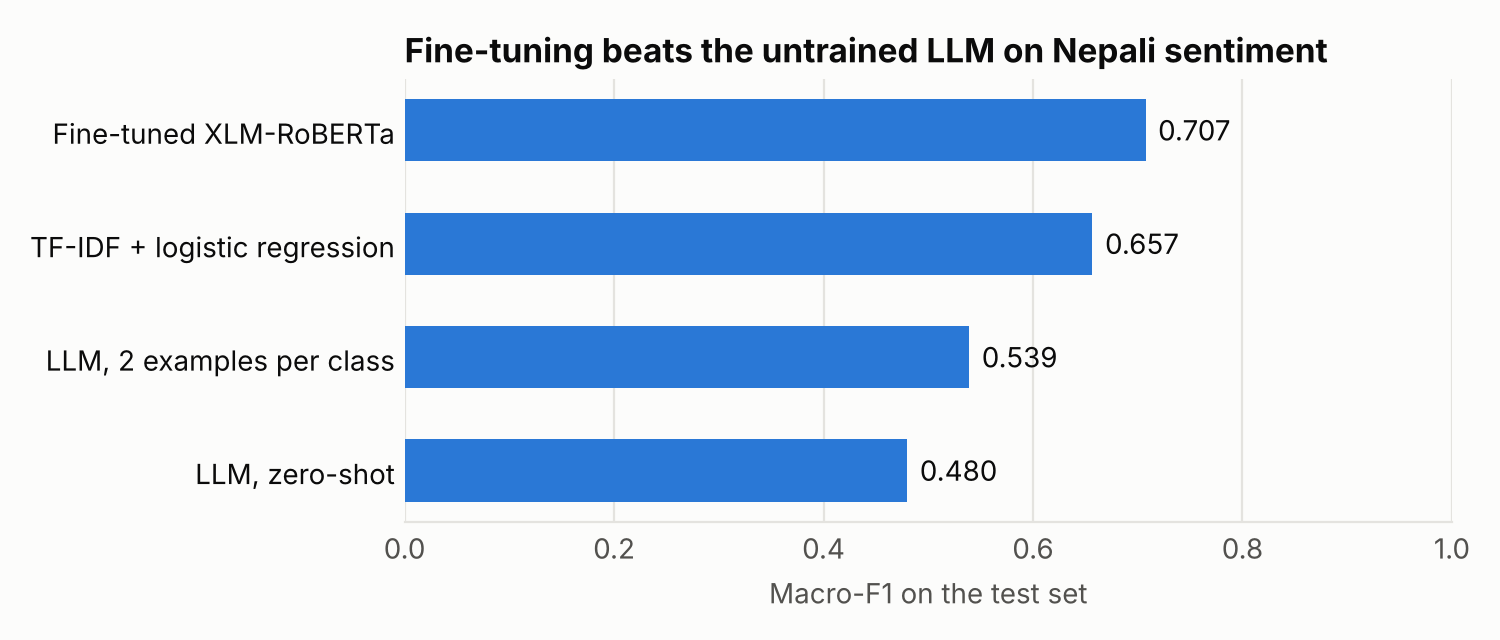
\includegraphics[width=\linewidth]{fig_macro_f1.png}\caption{Macro-F1}\end{subfigure}
\begin{subfigure}{0.49\textwidth}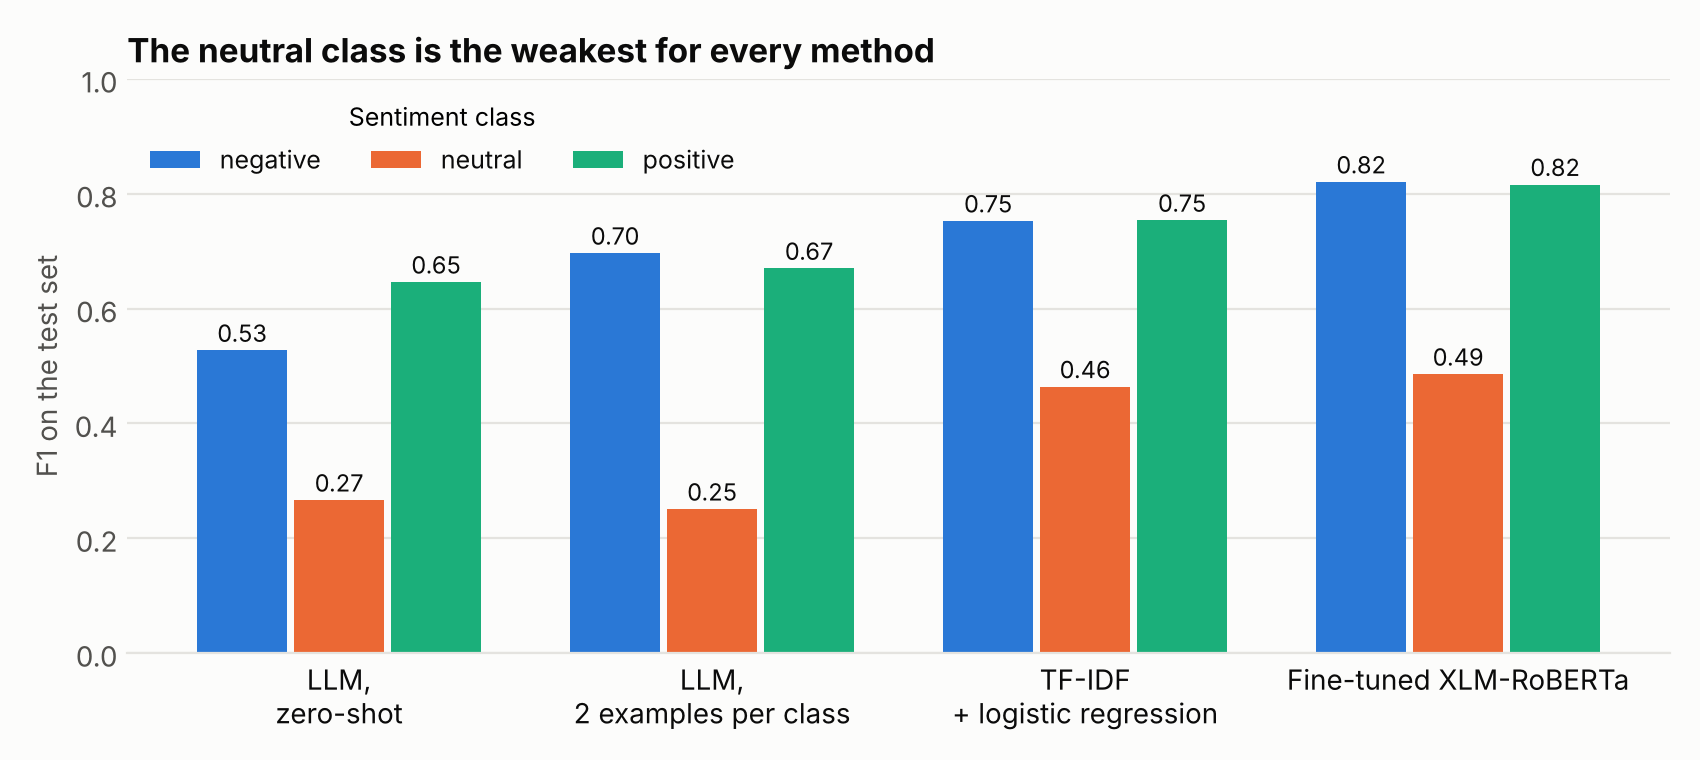
\includegraphics[width=\linewidth]{fig_per_class_f1.png}\caption{F1 per class}\end{subfigure}
\caption{Test-set scores by method.}
\label{fig:scores}
\end{figure}

\textbf{The LLM's errors are biased.} The confusion matrices (Fig.~\ref{fig:cm}) show that the LLM does not simply make more random mistakes. Zero-shot it called 581 of 1,360 negative tweets positive: negative recall was only 0.42 while positive recall was 0.75. With six examples the bias reversed: negative recall rose to 0.82, but 479 of 1,499 positive tweets were now called negative. A handful of examples moved the decision boundary a long way, in both directions.

\begin{figure}[H]
\centering
\begin{subfigure}{0.32\textwidth}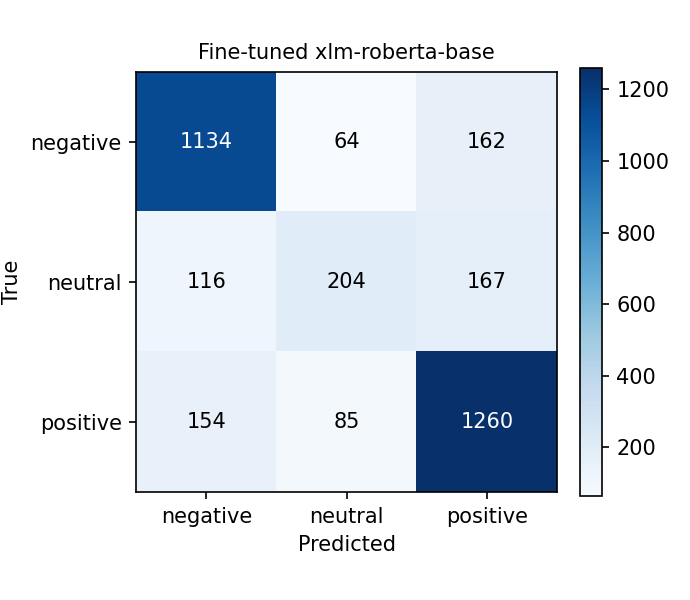
\includegraphics[width=\linewidth]{finetuned_xlm_roberta_base_confusion.png}\caption{XLM-R fine-tuned}\end{subfigure}
\begin{subfigure}{0.32\textwidth}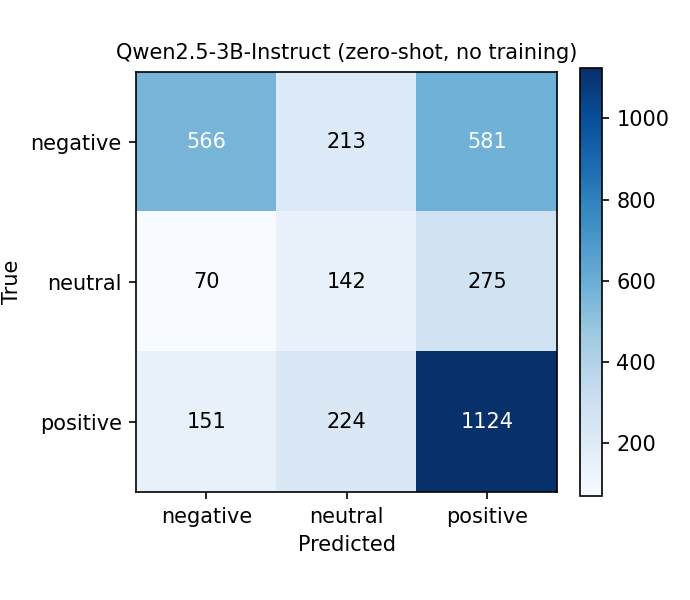
\includegraphics[width=\linewidth]{llm_qwen2_5_3b_instruct_0shot_confusion.png}\caption{LLM zero-shot}\end{subfigure}
\begin{subfigure}{0.32\textwidth}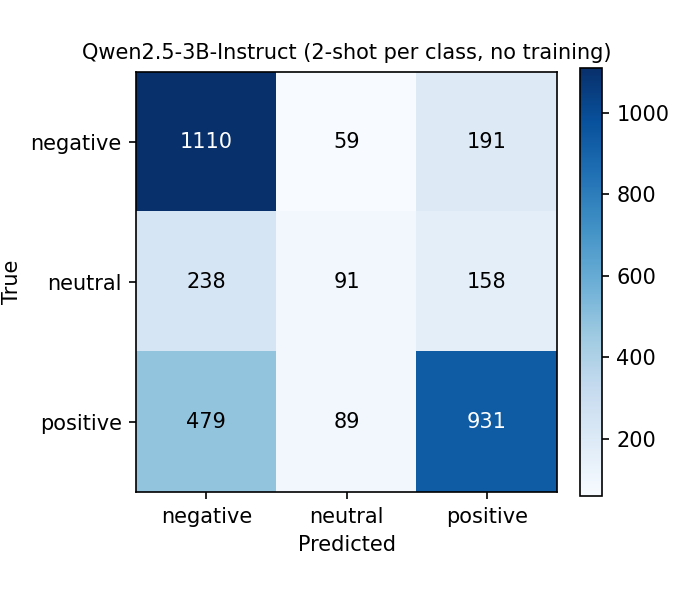
\includegraphics[width=\linewidth]{llm_qwen2_5_3b_instruct_2shot_confusion.png}\caption{LLM 2 per class}\end{subfigure}
\caption{Confusion matrices on the test set (rows: true label; columns: prediction).}
\label{fig:cm}
\end{figure}

\textbf{Neutral is hard for everyone.} No method exceeded 0.49 F1 on neutral tweets. Even the fine-tuned model labelled 167 of 487 neutral tweets positive and 116 negative, and got only 204 right. Neutral is the smallest class, but the TF-IDF model, trained with balanced class weights, did no better (0.46), which suggests that the problem lies at least partly in how neutral was labelled.

\textbf{Longer tweets are harder.} All four methods lost accuracy as tweets got longer (Fig.~\ref{fig:length}). For the fine-tuned model macro-F1 fell from 0.79 on tweets of up to 10 words to 0.60 on those over 40 words. Longer tweets more often mix several topics and opinions, which makes a single label harder to assign.

\begin{figure}[H]
\centering
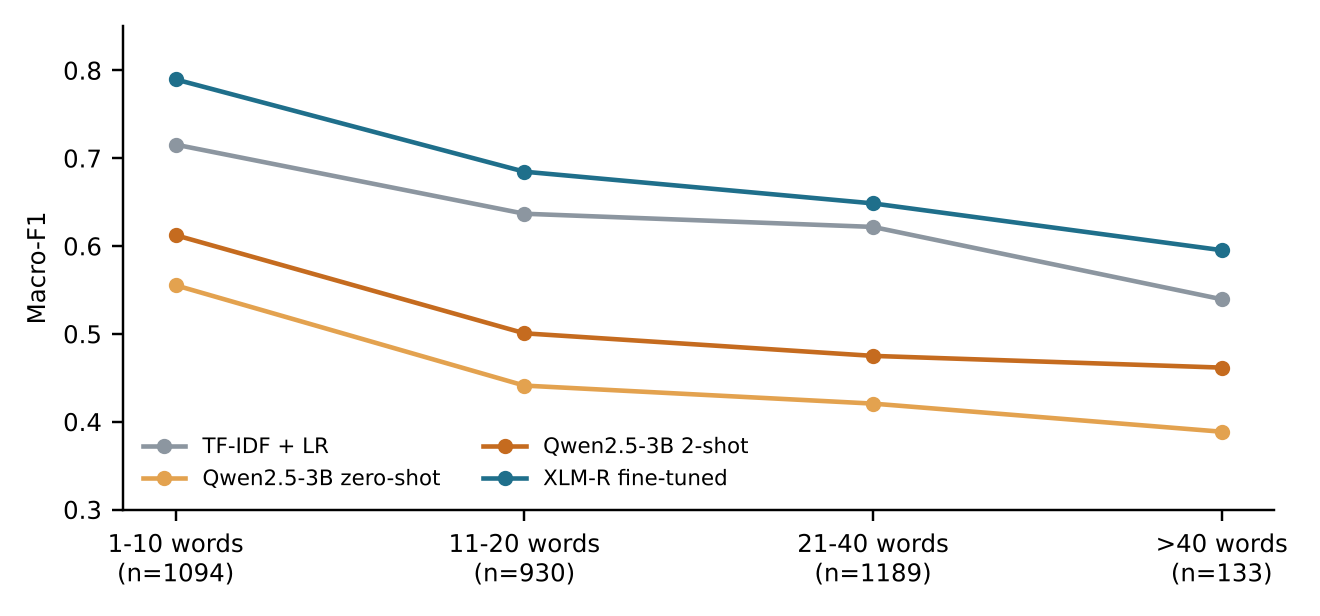
\includegraphics[width=0.72\textwidth]{fig_length.png}
\caption{Macro-F1 by tweet length on the test set.}
\label{fig:length}
\end{figure}

\textbf{Cost.} Fine-tuning took 13 minutes on one T4 GPU. Labelling the test set took the LLM 5.2 minutes zero-shot and 19.6 minutes with examples, since the examples make every prompt longer. The TF-IDF model trains in about a minute on a CPU.

\section{Discussion}

The answer to the question in the title is yes. With a few tens of thousands of labelled tweets, which is what most Nepali text-classification datasets offer, a fine-tuned encoder is better, cheaper to run and more predictable than a small open LLM used without training. The LLM is not useless: with no labels at all it gets more than half the tweets right, which may be enough to bootstrap labelling. But it should not be used as a classifier on its own.

Two findings are worth stressing for anyone using LLMs in a low-resource language. First, the LLM's errors are systematic, and a few prompt examples can flip them; any deployment would need checking on the target data, not just a headline accuracy. Second, even a character n-gram model beat the LLM, so a cheap baseline should always be part of the comparison.

\section{What can be explored next}
\begin{itemize}
\item \textbf{Larger and Nepali-aware models.} Repeat the comparison with 7B--70B open LLMs, with proprietary models, and with Nepali-specific encoders such as NepBERTa \cite{timilsina2022}.
\item \textbf{Prompt language.} Give the instruction in Nepali instead of English, and test more and better-chosen examples.
\item \textbf{Fine-tuning the LLM.} Parameter-efficient fine-tuning (for example LoRA) of the same 3B model would separate the effect of model size from the effect of training.
\item \textbf{Learning curves.} Fine-tune on 100, 500 and 2,000 labels to find the point at which fine-tuning overtakes the LLM.
\item \textbf{The neutral class.} Re-annotate a sample of neutral tweets with several annotators to measure label agreement.
\item \textbf{Other tasks and domains.} Disaster reports, news topics and hate speech in Nepali.
\end{itemize}

\section{Limitations}
One dataset and one domain (COVID-19 tweets); one random seed for fine-tuning, which can matter for transformers \cite{dodge2020}; one LLM and one prompt; and subjective labels. Differences of a point or less should not be read as meaningful.

\section{Conclusion}
On a leakage-free split of Nepali COVID-19 tweets, fine-tuned XLM-RoBERTa reached 0.707 macro-F1, a character n-gram baseline 0.657, and a 3B-parameter instruction-tuned LLM 0.480 zero-shot and 0.539 with six examples. For Nepali sentiment classification, fine-tuning a multilingual encoder remains the better choice, and the LLM's biased errors are a reason for caution beyond its lower scores.

\section*{Data and code availability}
The dataset is public on the Hugging Face Hub (\texttt{raygx/NepCov19Tweets}) and belongs to its original authors. All code, metrics, per-tweet predictions and figures are at \url{https://github.com/subarna007/nepali-sentiment-finetune-vs-llm}.

\begin{thebibliography}{99}\small
\bibitem{joshi2020} Joshi P, Santy S, Budhiraja A, Bali K, Choudhury M. The state and fate of linguistic diversity and inclusion in the NLP world. In: ACL 2020. p. 6282--6293.
\bibitem{conneau2020} Conneau A, Khandelwal K, Goyal N, Chaudhary V, Wenzek G, Guzm\'an F, et al. Unsupervised cross-lingual representation learning at scale. In: ACL 2020. p. 8440--8451.
\bibitem{brown2020} Brown T, Mann B, Ryder N, Subbiah M, Kaplan J, Dhariwal P, et al. Language models are few-shot learners. In: NeurIPS 2020.
\bibitem{ahuja2023} Ahuja K, Diddee H, Hada R, Ochieng M, Ramesh K, Jain P, et al. MEGA: multilingual evaluation of generative AI. In: EMNLP 2023.
\bibitem{lai2023} Lai VD, Ngo NT, Pouran Ben Veyseh A, Man H, Dernoncourt F, Bui T, et al. ChatGPT beyond English: towards a comprehensive evaluation of large language models in multilingual learning. In: Findings of EMNLP 2023.
\bibitem{zhang2023} Zhang W, Deng Y, Liu B, Pan SJ, Bing L. Sentiment analysis in the era of large language models: a reality check. arXiv:2305.15005; 2023.
\bibitem{sitaula2021} Sitaula C, Basnet A, Mainali A, Shahi TB. Deep learning-based methods for sentiment analysis on Nepali COVID-19-related tweets. Computational Intelligence and Neuroscience. 2021;2021:2158184. doi: 10.1155/2021/2158184
\bibitem{wolf2020} Wolf T, Debut L, Sanh V, Chaumond J, Delangue C, Moi A, et al. Transformers: state-of-the-art natural language processing. In: EMNLP 2020: System Demonstrations. p. 38--45.
\bibitem{qwen2024} Qwen Team. Qwen2.5 technical report. arXiv:2412.15115; 2024.
\bibitem{efron1993} Efron B, Tibshirani RJ. An introduction to the bootstrap. Chapman and Hall; 1993.
\bibitem{mcnemar1947} McNemar Q. Note on the sampling error of the difference between correlated proportions or percentages. Psychometrika. 1947;12(2):153--157.
\bibitem{dietterich1998} Dietterich TG. Approximate statistical tests for comparing supervised classification learning algorithms. Neural Computation. 1998;10(7):1895--1923.
\bibitem{timilsina2022} Timilsina S, Gautam M, Bhattarai B. NepBERTa: Nepali language model trained in a large corpus. In: AACL-IJCNLP 2022.
\bibitem{dodge2020} Dodge J, Ilharco G, Schwartz R, Farhadi A, Hajishirzi H, Smith N. Fine-tuning pretrained language models: weight initializations, data orders, and early stopping. arXiv:2002.06305; 2020.
\end{thebibliography}

\end{document}
